\documentclass[a4paper,10pt]{article}
\usepackage[utf8]{inputenc}
\usepackage{graphicx}

%opening
\title{}
\author{}

\begin{document}

\maketitle

\begin{abstract}

\end{abstract}


\section{Partie 1 : Analyse et Spécification des besoins}
\subsection{Buts et destinataires}
L'objectif de ce projet est de centraliser et informatiser les factures au sein d'une entreprise.
Avec pour objectif d'accélérer les remboursements.

\subsection{Définition-Abréviation}
\begin{enumerate}
\item{OCR} (Optical Character Recognition) Reconnaissance active de caractères.
\end{enumerate}

\subsection{Présentation générale du document}


\section{Partie 2 : Description Générale}
\subsection{Environnement ou contexte du système}
FactureOCR sera situé au sein du service comptabilité de l'entreprise.
Il n'est en relation avec aucun autre système de l'entreprise étant donné que sa base de données est indépendante.

Un seul Acteur interagit avec le système : l'utilisateur. Le système communique avec une base de données intégrée. 

\subsection{Modèle Conceptuel}
Les principales fonctions du système sont le chargement, l'extraction et la modification des données présentes dans les factures et les tickets de caisses ainsi que l'enregistrement.

\begin{figure}[!ht] %on ouvre l'environnement figure
  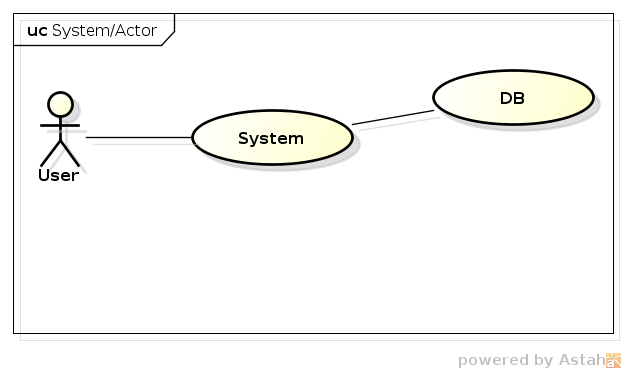
\includegraphics[width=5cm]{SystemActor.png} %ou image.png, .jpeg etc.
  \caption{testl} %la légende
  \label{test} %l'étiquette pour faire référence à cette image
\end{figure} %on ferme l'environnement figure


\section{Les besoins en performance}

\subsection{Nombre maximum de terminaux}

Le nombre maximum de terminaux n’est pas pertinent dans ce projet. L’intégralité des calculs 

est effectuée du côté client, et la base de données est stockée localement. Si cette dernière est 

distante, le nombre de requêtes étant très limité, une somme importante de clients n’est pas un 

souci.

\subsection{Nombre maximum de transactions simultanées}

Le nombre d’accès à la base de données (partie potentiellement commune aux clients) est très 

réduit. De ce fait, un nombre maximum de transactions simultanées à la base de données de 1 

n’est pas un problème.

\subsection{Nombre de fichiers et leurs tailles}

Pour chaque facture / ticket de caisse considéré, il y a un fichier image (jusqu’à 10 Mo), un 

fichier texte contenant les données récupérées (200 Ko maximum) et un autre contenant les 

modifications apportées par l’utilisateur (taille inférieure au premier fichier texte). Un modèle 

de facture / ticket de caisse doit être aussi présent pour chaque type de document ; stocké sous 

forme textuelle, sa taille ne dépasse pas 500 Ko.

Au total, en moyenne, pour une somme de 1000 factures, un espace de stockage de 5 Go doit 

être alloué.

\subsection{Temps de réponse souhaité}

Les accès à la base de données ne sont pas cruciaux en termes de durée. La lecture et 

l’écriture ne doivent pas être très lentes, mais un temps de réponse élevé (une seconde 

maximum) reste convenable. Cependant, la partie extraction et affichage des données ne 

doit pas être mal optimisée, car les technologies utilisées (OCR) peuvent être rapidement 

gourmandes en temps et capacité de calcul si elles sont poussives.

\subsection{Les contraintes liées à l'environnement (temps réel)}

Il n’y a pas de contrainte d’exécution temps réel, si ce n’est un temps de réponse excessif de 

l’application. Un ordinateur standard (voire tablette ou smartphone) sera capable de supporter 

la charge de travail demandée par l’application avec un délai raisonnable, avec ou sans base 

de données distante.

Développé de manière portable, le logiciel devra être exécutable depuis une machine 

Windows ou Unix (Linus ou Mac).

\section{ Les contraintes de développement}

\subsection{Fiabilité et tolérance aux fautes}

La reconnaissance optique de caractères ne peut pas donner de résultats fiables pour n’importe 

quelle entrée. De ce fait, la partie vérification des erreurs est majoritairement réalisée par 

l’utilisateur, via la phase de correction et d’enregistrement dans la base de données. L’image 

dont les données sont extraites est aussi stockée, laissant la possibilité d’une vérification 

ultérieure.

\subsection{Le comportement du système dans des situations anormales (les exceptions critiques)}

Lorsqu’une urgence survient, le logiciel doit être en mesure de prévenir l’utilisateur et de ne 

pas transmettre de données erronées. 

\subsection{Sécurité}

Si les données présentes dans les factures sont sensibles, la mise en place de protocoles de 

transmission sécurisés et de chiffrage des données stockées peut être réalisée.

\subsection{Restriction sur l'utilisation de certaines commandes}

Certaines fonctions (notamment récupération et/ou édition d’informations présentes dans la 

base de données) doivent pouvoir être limitées à certains utilisateurs.

\subsection{Contrôle des accès aux données}

Comme écrit ci-dessus, certains utilisateurs peuvent n’avoir besoin que de l’affichage de 

certaines données. L’accès à d’autres et la modification doivent pouvoir être contrôlées, soit 

par des fonctions restreintes en fonction de l’utilisateur, soit par des enregistrements des 

activités et des vérifications de ces dernières.

\subsection{Utilisation de mot de passe}

Si les problèmes de sécurité discutés ci-dessus sont présents, un système de mot de passe 

ou de carte magnétique doit pouvoir être instauré afin de respecter les contraintes citées 

précédemment.

\subsection{Utilisation de standards en ce qui concerne les méthodes, outils et langages de développement.}

Le logiciel fourni doit pouvoir être portable et fonctionnel. Il doit être réutilisable et donc 

modulaire. Un environnement de travail à licence permissive doit être adopté, ainsi que des 

langages de développement libres d’utilisations.



\end{document}


